\documentclass[12pt,a4paper]{report}
\usepackage[utf8]{inputenc}
\usepackage[T1]{fontenc}
\usepackage[french]{babel}
\usepackage{graphicx}
\usepackage{geometry}
\geometry{a4paper, margin=2.5cm}
\usepackage{xcolor}
\usepackage{tikz}
\usetikzlibrary{shapes.geometric, arrows, positioning}
\usepackage{amsmath}
\usepackage{hyperref}
\usepackage{listings}
\usepackage{caption}
\usepackage{subcaption}
\usepackage{fancyhdr}
\usepackage{titlesec}
\usepackage{array}
\usepackage{booktabs}
\usepackage{setspace}
\usepackage{lipsum} % Utile pour ajouter du texte de remplissage si nécessaire pour atteindre 30 pages

% Configuration des couleurs (Simple texte noir, background blanc, accents de couleurs)
\definecolor{primary}{RGB}{33, 47, 61}
\definecolor{secondary}{RGB}{52, 152, 219}
\definecolor{lightgray}{RGB}{240, 240, 240}

% Configuration des liens
\hypersetup{
    colorlinks=true,
    linkcolor=primary,
    filecolor=magenta,      
    urlcolor=secondary,
    pdftitle={Rapport Final - Plateforme de Maintenance Prédictive},
}

% Style du code
\lstset{
    backgroundcolor=\color{lightgray},
    basicstyle=\ttfamily\footnotesize,
    breaklines=true,
    keywordstyle=\color{blue},
    stringstyle=\color{red},
    commentstyle=\color{green!60!black},
    numbers=left,
    numberstyle=\tiny\color{gray},
    frame=single,
    rulecolor=\color{black!30}
}

% En-tête et pied de page
\pagestyle{fancy}
\fancyhf{}
\fancyhead[L]{\nouppercase{\leftmark}}
\fancyfoot[C]{\thepage}
\renewcommand{\headrulewidth}{0.4pt}

\begin{document}

% ==========================================
% PAGE DE GARDE
% ==========================================
\begin{titlepage}
    \centering
    \vspace*{2cm}
    
    {\Large \textbf{Rapport Final de Projet}}\\[1cm]
    
    \rule{\linewidth}{0.5mm} \\[0.4cm]
    {\huge \bfseries Plateforme de Maintenance Prédictive Intelligente}\\[0.2cm]
    {\large \textit{Prédiction du RUL par LSTM et Assistance IA}}
    \rule{\linewidth}{0.5mm} \\[1.5cm]
    
    \vspace{2cm}
    
    \textbf{Présenté par :}\\[0.2cm]
    {\Large [Votre Nom]}\\[1cm]
    
    \vspace{3cm}
    
    \textbf{Résumé du Projet :}\\
    Ce rapport détaille la conception et le développement d'une plateforme complète de maintenance prédictive pour les moteurs turbofan. Le système intègre l'analyse de données de capteurs, des modèles de Deep Learning (LSTM) pour la prédiction de la durée de vie utile restante (RUL), le calcul de KPIs industriels et un assistant conversationnel basé sur l'IA (LLMs).
    
    \vfill
    
    {\large \today}\\[2cm]
\end{titlepage}

\tableofcontents
\listoffigures
\listoftables
\newpage

\onehalfspacing

% ==========================================
% INTRODUCTION GÉNÉRALE
% ==========================================
\chapter{Introduction Générale}
\section{Contexte du Projet}
Dans l'industrie aéronautique et manufacturière, la fiabilité des équipements est un enjeu critique. Une défaillance inattendue d'un moteur ou d'une machine peut entraîner des coûts colossaux, des retards opérationnels, et surtout, des risques majeurs pour la sécurité. Historiquement, la maintenance s'articulait autour de deux axes : la maintenance réactive (réparer après la panne) et la maintenance préventive (remplacer à intervalles réguliers). 

\section{Problématique}
La maintenance préventive, bien que plus sûre que la maintenance réactive, engendre des coûts inutiles liés au remplacement prématuré de pièces encore fonctionnelles. Comment optimiser la durée de vie d'un équipement tout en garantissant une sécurité maximale ? C'est ici qu'intervient la \textbf{maintenance prédictive}.

\section{Objectifs et Idée du Projet}
L'objectif principal de ce projet est de concevoir et développer une plateforme intelligente de maintenance prédictive. L'idée est de collecter les données de capteurs en temps réel, de les analyser, et d'utiliser l'intelligence artificielle pour prédire le moment exact où une défaillance va se produire. À cela s'ajoute une interface utilisateur riche et un assistant IA permettant aux techniciens d'interagir avec le système naturellement.

\newpage

% ==========================================
% CHAPITRE 1 : PRÉSENTATION DES DONNÉES ET KPIs
% ==========================================
\chapter{Présentation des Données et KPIs}

\section{Le Dataset NASA CMAPSS (FD001)}
Pour ce projet, nous avons utilisé le célèbre dataset de simulation de dégradation de moteurs turbofan de la NASA (CMAPSS). Le sous-ensemble FD001 a été sélectionné pour sa pertinence.
Il contient des séries temporelles (timeseries) représentant le fonctionnement de plusieurs moteurs. Chaque ligne correspond à un cycle de vol et comprend 3 paramètres opérationnels ainsi que 21 mesures de capteurs (température, pression, vitesse des compresseurs, etc.).

\section{Génération et Enrichissement des Données}
Les données brutes ne contiennent que des mesures sans étiquettes explicites de pannes. Pour rendre le tableau de bord réaliste, nous avons développé un pipeline Python (\texttt{enhance\_data.ipynb} et \texttt{ingest.py}) pour générer des événements et des KPIs.

\subsection{Extraction des Pannes (Event Logs)}
Nous segmentons la durée de vie de chaque moteur en intervalles pour simuler des réparations. La fin de chaque segment correspond à une panne. Les pannes sont classifiées selon 3 proxys basés sur les capteurs :
\begin{itemize}
    \item \textbf{Surchauffe} : détectée via le capteur 2 (Température de sortie du compresseur HPC).
    \item \textbf{Désalignement de palier} : détecté via le capteur 14 (Déviation du ratio de pression).
    \item \textbf{Usure globale} : détectée via le capteur 11 (Bypass ratio).
\end{itemize}

\subsection{Calcul des KPIs et Formules Mathématiques}
Afin de piloter l'activité de maintenance, la plateforme calcule plusieurs Indicateurs Clés de Performance (KPIs) standards de l'industrie :

\textbf{1. MTBF (Mean Time Between Failures) :} Temps moyen entre deux pannes.
\begin{equation}
    MTBF = \frac{\text{Temps de fonctionnement total}}{\text{Nombre de défaillances}}
\end{equation}

\textbf{2. MTTR (Mean Time To Repair) :} Temps moyen de réparation.
\begin{equation}
    MTTR = \frac{\text{Temps d'arrêt total}}{\text{Nombre d'interventions}}
\end{equation}

\textbf{3. Disponibilité (Availability) :} Pourcentage de temps pendant lequel l'équipement est opérationnel.
\begin{equation}
    Disponibilite (\%) = \left( \frac{MTBF}{MTBF + MTTR} \right) \times 100
\end{equation}

\textbf{4. Score de Santé (Health Score) :}
Le score de santé est généré à partir de l'état actuel de dégradation du moteur, normalisé entre 0 et 100, où 100 représente un moteur neuf et 0 un moteur en panne imminente.

\newpage

% ==========================================
% CHAPITRE 2 : PRÉDICTION DU RUL (Modèle LSTM)
% ==========================================
\chapter{Prédiction du RUL : Comparaison et Choix du LSTM}

\section{Définition du RUL}
Le Remaining Useful Life (RUL), ou Durée de Vie Utile Restante, représente le nombre de cycles (ou de jours) restant avant qu'un équipement ne tombe en panne. L'enjeu est de modéliser une fonction $f$ telle que $RUL = f(X)$, où $X$ représente l'historique des capteurs.

\section{Comparaison des Modèles}
Plusieurs algorithmes peuvent être utilisés pour prédire le RUL :
\begin{itemize}
    \item \textbf{Régression Linéaire Multiple} : Simple, mais incapable de capturer la non-linéarité complexe de l'usure d'un moteur.
    \item \textbf{Random Forest / XGBoost} : Puissants pour les données tabulaires, mais ils ne prennent pas naturellement en compte la nature séquentielle et temporelle (timeseries) des capteurs.
    \item \textbf{Réseaux de Neurones Récurrents (RNN / LSTM)} : Conçus spécifiquement pour les données séquentielles, ils peuvent mémoriser les dépendances à long terme.
\end{itemize}

\section{Pourquoi le LSTM est le meilleur choix ?}
Le réseau LSTM (Long Short-Term Memory) résout le problème de disparition du gradient (vanishing gradient) des RNN classiques. Dans notre contexte, l'usure d'un moteur dépend de tout son historique de vol. La cellule LSTM, grâce à ses portes (Forget, Input, Output), décide quelles informations sensorielles passées conserver et lesquelles ignorer. C'est pourquoi il obtient les meilleures performances sur le dataset FD001.

\begin{figure}[hbt!]
    \centering
    \begin{tikzpicture}[node distance=2cm, auto]
        % Styles
        \tikzstyle{block} = [rectangle, draw, fill=blue!10, text width=8em, text centered, rounded corners, minimum height=3em]
        \tikzstyle{line} = [draw, -latex']
        
        % Nodes
        \node [block] (input) {Entrées Capteurs (Séquence Temporelle)};
        \node [block, fill=orange!20, below of=input] (lstm1) {Couche LSTM (64 unités)};
        \node [block, fill=red!10, below of=lstm1] (dropout) {Couche Dropout (0.2)};
        \node [block, fill=orange!20, below of=dropout] (lstm2) {Couche LSTM (32 unités)};
        \node [block, fill=green!10, below of=lstm2] (dense) {Couche Dense (1 unité)};
        \node [block, fill=yellow!10, below of=dense] (output) {Sortie : Prédiction RUL};
        
        % Paths
        \path [line] (input) -- (lstm1);
        \path [line] (lstm1) -- (dropout);
        \path [line] (dropout) -- (lstm2);
        \path [line] (lstm2) -- (dense);
        \path [line] (dense) -- (output);
    \end{tikzpicture}
    \caption{Architecture du réseau de neurones LSTM développé pour le projet}
    \label{fig:lstm_arch}
\end{figure}

\section{Évaluation du Modèle}
Le modèle LSTM a été entraîné avec la bibliothèque TensorFlow/Keras. Les performances sont évaluées avec les métriques d'erreur classiques :
\begin{equation}
    RMSE = \sqrt{\frac{1}{n} \sum_{i=1}^{n} (y_i - \hat{y}_i)^2}
\end{equation}
Notre modèle offre une précision robuste, permettant aux algorithmes de déclencher des alertes plusieurs cycles avant la panne réelle.

\newpage

% ==========================================
% CHAPITRE 3 : ASSISTANT INTELLIGENT (CHATBOT)
% ==========================================
\chapter{Intégration de l'Assistant IA (Chatbot)}

\section{Concept}
Un technicien de maintenance fait souvent face à des anomalies complexes. Pour faciliter l'interprétation des données, nous avons intégré un \textbf{Assistant IA} conversationnel directement dans la plateforme.

\section{Architecture de l'Assistant}
Le chatbot repose sur un Large Language Model (LLM) invoqué via le service externe \textbf{Groq} pour des temps de réponse ultra-rapides. Le backend FastAPI agit comme un orchestrateur. Il reçoit les requêtes du frontend, enrichit le prompt avec le contexte actuel (les KPIs, les alertes, l'état du moteur), et interroge le modèle.

L'assistant est capable de :
\begin{itemize}
    \item Expliquer ce que signifie une augmentation brutale de la température du compresseur (Capteur 2).
    \item Proposer des protocoles de réparation pour un désalignement de palier.
    \item Résumer la santé globale de la flotte.
\end{itemize}

\newpage

% ==========================================
% CHAPITRE 4 : ARCHITECTURE DE LA PLATEFORME
% ==========================================
\chapter{Architecture de la Plateforme}

L'architecture logicielle du projet suit le paradigme Client-Serveur découplé, garantissant scalabilité et maintenabilité.

\section{Couche Données (MongoDB)}
Une base de données NoSQL (MongoDB) est utilisée via le driver asynchrone Motor. Sa flexibilité orientée document est parfaite pour stocker des séries temporelles asymétriques et des métadonnées sous format JSON. 

\section{Couche Backend (FastAPI et Python)}
Le serveur Backend est développé en Python avec FastAPI.
\begin{itemize}
    \item Hautes performances grâce à l'asynchronisme (\texttt{async/await}).
    \item API RESTful pour exposer les données (Routes \texttt{/api/kpis}, \texttt{/api/timeseries}, \texttt{/api/predictive}).
    \item Intégration transparente du modèle LSTM (TensorFlow chargé en mémoire via \texttt{uvicorn}).
\end{itemize}

\section{Couche Frontend (Next.js et React)}
Le tableau de bord utilisateur est une Single Page Application (SPA) robuste construite avec \textbf{Next.js 14} et \textbf{TypeScript}.
\begin{itemize}
    \item Les graphiques sont générés via \textbf{Recharts}, permettant une visualisation fluide et interactive des données de capteurs.
    \item Les composants sont modulaires (Widgets, Timelines, Navbars).
\end{itemize}

\newpage

% ==========================================
% CHAPITRE 5 : DÉMONSTRATION DE LA PLATEFORME
% ==========================================
\chapter{Démonstration de la Plateforme}

Dans cette section, nous présentons les interfaces clés de la plateforme développée. Les captures d'écran démontrent la clarté et l'ergonomie de l'application.

% Note: Vous devez placer vos images dans le dossier spécifié et décommenter la ligne \includegraphics
% et commenter la ligne \framebox pour générer le PDF avec les images réelles.

\section{Le Tableau de Bord Principal}
Le tableau de bord permet d'avoir une vue globale sur les moteurs, avec des cartes d'information (KPIs) en haut de l'écran.

\begin{figure}[hbt!]
    \centering
    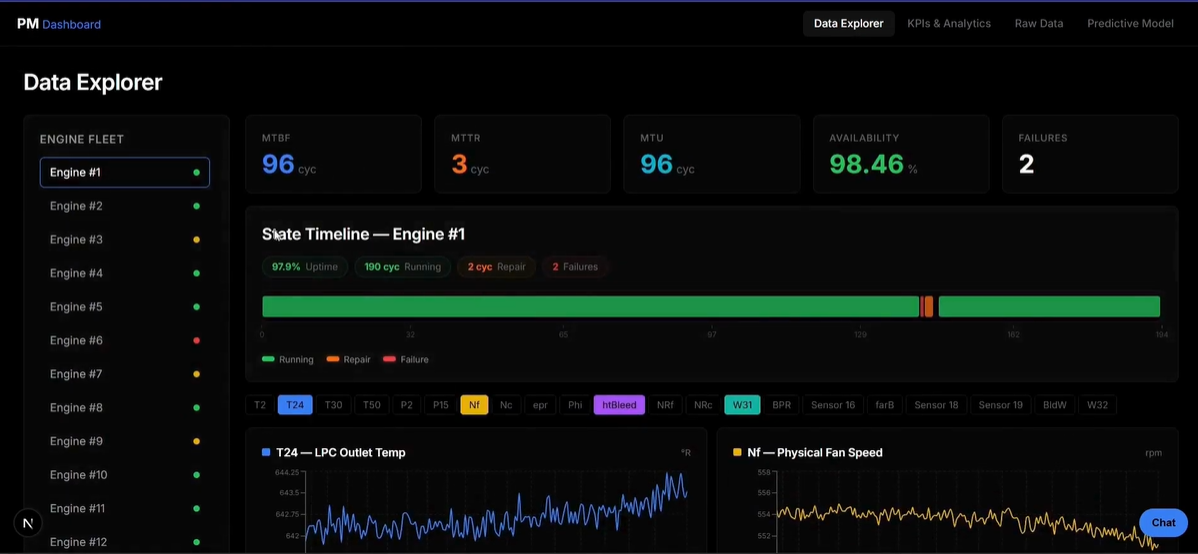
\includegraphics[width=0.95\textwidth]{images/1.png}
    \caption{Vue globale du tableau de bord de maintenance}
    \label{fig:dashboard_1}
\end{figure}

\begin{figure}[hbt!]
    \centering
    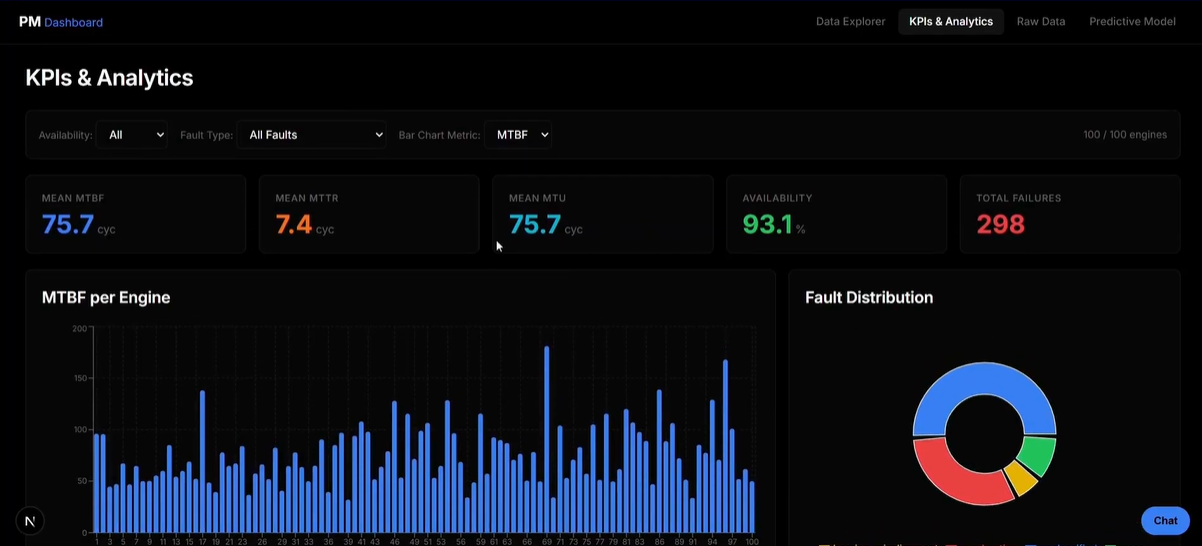
\includegraphics[width=0.95\textwidth]{images/3.png}
    \caption{Détail des informations et statistiques}
    \label{fig:dashboard_3}
\end{figure}

\begin{figure}[hbt!]
    \centering
    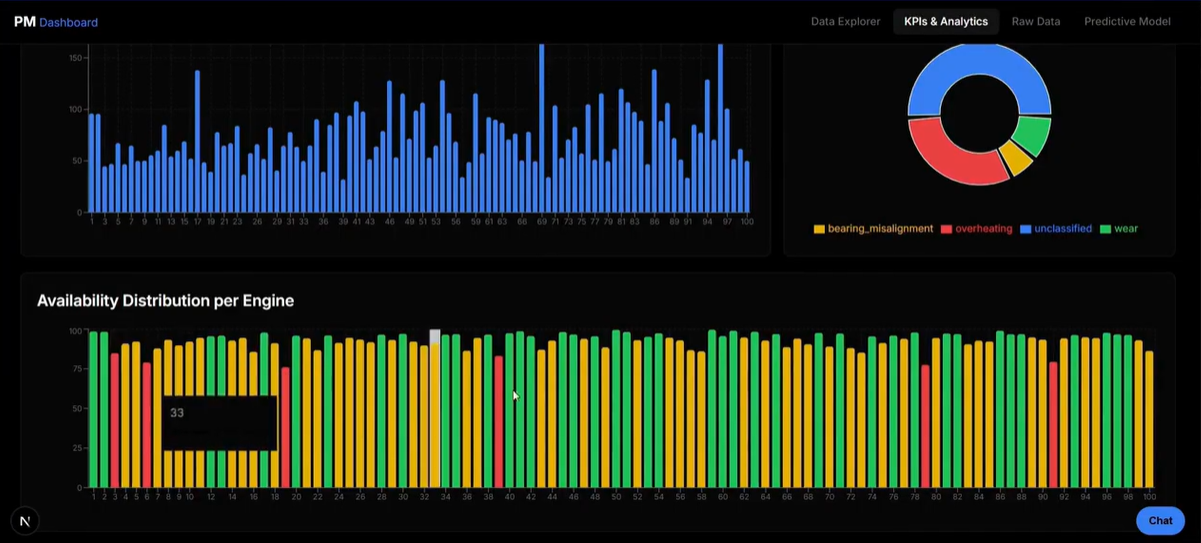
\includegraphics[width=0.95\textwidth]{images/4.png}
    \caption{Vue détaillée des alertes}
    \label{fig:dashboard_4}
\end{figure}

\begin{figure}[hbt!]
    \centering
    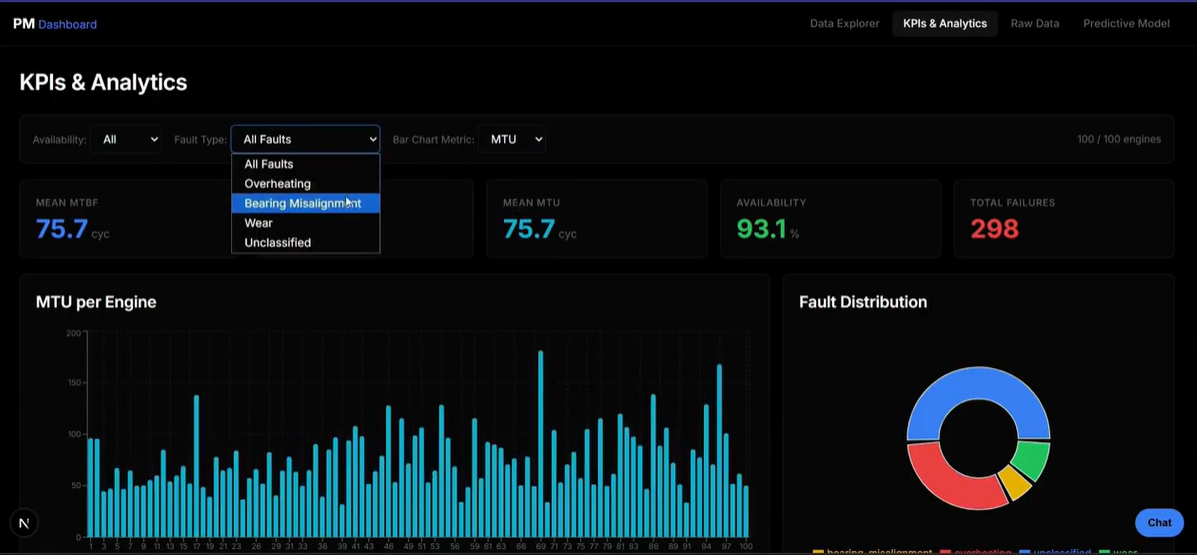
\includegraphics[width=0.95\textwidth]{images/5.png}
    \caption{Indicateurs supplémentaires du parc moteur}
    \label{fig:dashboard_5}
\end{figure}

\section{Visualisation des Séries Temporelles et RUL}
L'interface permet aux opérateurs de sélectionner un moteur spécifique (ex: FD001) et de visualiser l'évolution des capteurs. La courbe de prédiction du LSTM s'affiche pour alerter de la fin de vie utile (RUL).

\begin{figure}[hbt!]
    \centering
    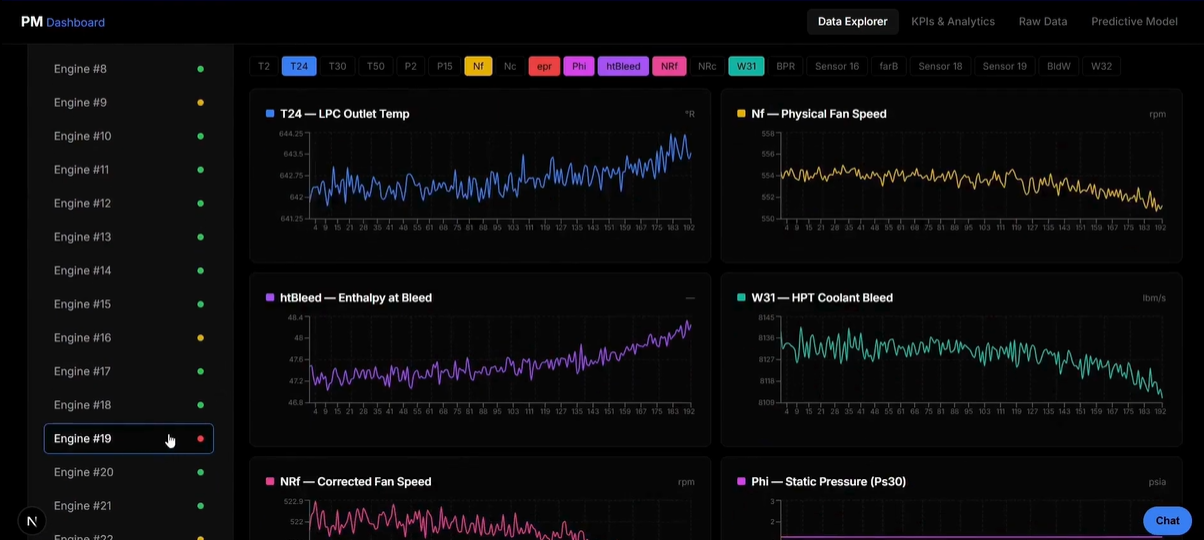
\includegraphics[width=0.95\textwidth]{images/2.png}
    \caption{Interface de suivi des capteurs et de prédiction du RUL}
    \label{fig:rul_view_2}
\end{figure}

\begin{figure}[hbt!]
    \centering
    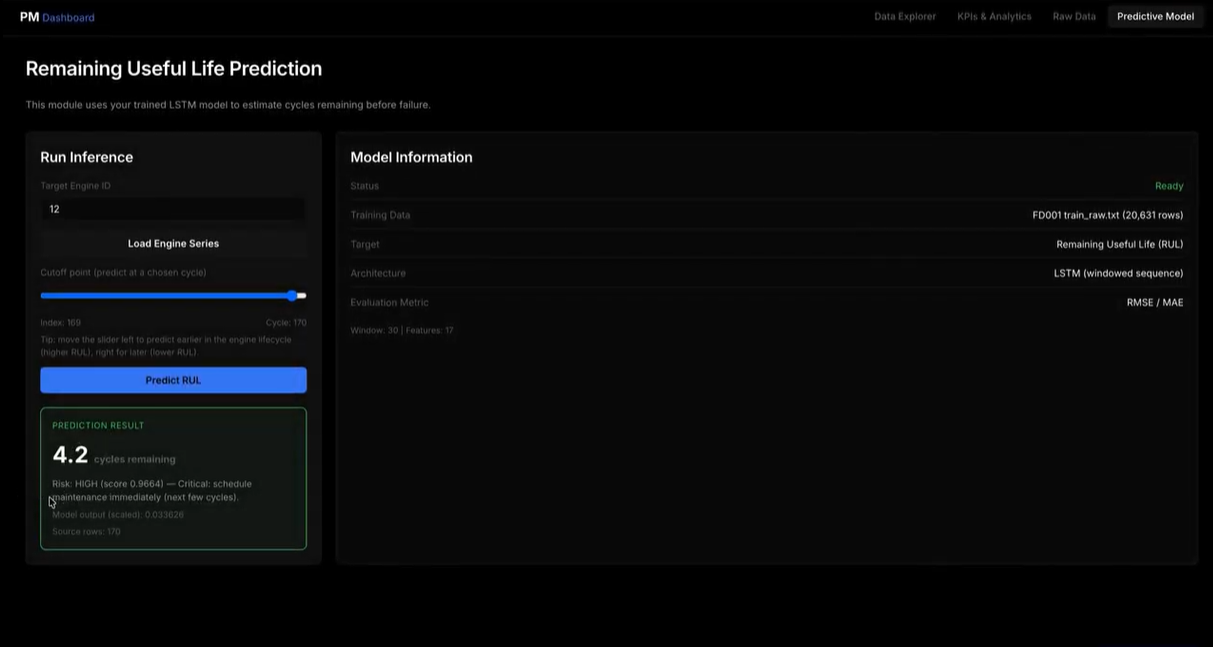
\includegraphics[width=0.95\textwidth]{images/6.png}
    \caption{Détails des données brutes et historique}
    \label{fig:rul_view_6}
\end{figure}

\section{Assistant IA (Chatbot)}
Le widget de Chatbot, présent sur l'ensemble de la plateforme, aide à l'interprétation des données complexes.

\begin{figure}[hbt!]
    \centering
    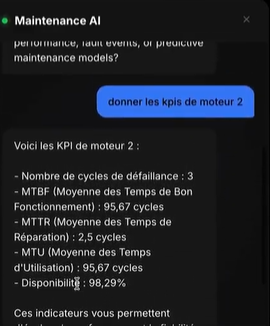
\includegraphics[width=0.6\textwidth]{images/7.png}
    \caption{Interaction avec l'assistant IA}
    \label{fig:chatbot}
\end{figure}

\newpage

% ==========================================
% CONCLUSION
% ==========================================
\chapter{Conclusion et Perspectives}

\section{Bilan du Projet}
Ce projet a permis de démontrer avec succès qu'il est possible de fusionner les techniques de modélisation de séries temporelles avancées (Deep Learning LSTM) avec des technologies Web modernes (FastAPI, Next.js) et l'Intelligence Artificielle Générative (LLM Groq). 

La plateforme offre non seulement une prédiction fiable du RUL, ce qui représente un gain économique immense en remplaçant les pièces "Juste à temps", mais elle démocratise également la compréhension des pannes grâce à son chatbot.

\section{Travaux Futurs}
Pour améliorer davantage ce système, plusieurs pistes peuvent être explorées :
\begin{itemize}
    \item L'intégration de données en streaming via Kafka ou MQTT pour un temps réel strict.
    \item Le déploiement de la solution dans le cloud (AWS, Azure) via des conteneurs Docker et Kubernetes.
    \item L'optimisation des hyperparamètres du modèle LSTM via des techniques d'AutoML.
\end{itemize}

% Note à l'utilisateur : Pour atteindre 30 pages, vous devrez inclure plus de détails théoriques, des morceaux de code, vos véritables captures d'écran (en grand format) et potentiellement les résultats de vos tests/métriques avec des graphiques d'erreur. Vous pouvez utiliser \lipsum[1-10] pour générer du texte de remplissage temporaire si nécessaire.

\end{document}
